\documentclass[class=article , crop=false, titlepage, twoside, multi={itemize, figure, verbatim}, float=false]{standalone}
\usepackage{caption}
\usepackage{import} % Required for importing other .tex docs.  (import uses everything bw Begin and End Doc)
\usepackage{float} % Required for specifying the exact location of a figure or table
\usepackage{graphicx} % Required for including images
\usepackage{wrapfig}
\usepackage[pdftex,breaklinks,colorlinks=true,linkcolor=black,citecolor=blue,urlcolor=red,linktocpage=false,pagebackref=true,filecolor=magenta]{hyperref}%http://www.tug.org/applications/hyperref/manual.html#x1-100003.6
\usepackage{cite}
\usepackage[toc,title,page]{appendix}
\usepackage{pdfpages} % enables loading a pdf into the doc
\usepackage{makeidx}
\usepackage{glossaries} % must be after hyperref
\usepackage{blindtext}
\usepackage{enumitem}
%\usepackage{caption}

%\setlist[description]{leftmargin=\parindent,labelindent=\parindent}

%\renewcommand*{\bibname}{References} % renames the bibliography

\newcommand{\HRule}{\rule{\linewidth}{0.5mm}} % Command to make the lines in the title page

\graphicspath{{img/}{GIS_ChampionSection/img/}{awardsChapter/GIS_ChampionSection/img/}{brandPart/awardsChapter/GIS_ChampionSection/img/}{img/}{pairedProgSection/img/}{methodChapter/pairedProgSection/img/}{methodPart/methodChapter/pairedProgSection/img/}{documentationSection/img/}{methodChapter/documentationSection/img/}{methodPart/methodChapter/documentationSection/img/}{docStorageOrgSection/img/}{methodChapter/docStorageOrgSection/img/}{methodPart/methodChapter/docStorageOrgSection/img/}{QGisSection/img/}{toolsChapter/QGisSection/img/}{servicePart/toolsChapter/QGisSection/img/}{ESRISection/img/}{toolChapter/ESRISection/img/}{servicePart/toolChapter/ESRISection/img/}{../../../../source/}{../../source/}{servicePart/applicationsChapter/treasurerSection/img/}}

%\setlength\parindent{0pt} % eliminates indents


\def\titlename{Forfeiture Data Collection\\ \medskip\large Mobile App with Collector for ArcGIS}

\title{\HRule % Horizontal Line added
\\[.4cm] % space
\begin{figure}[H] % included image
\begin{center}	% centered horizontally
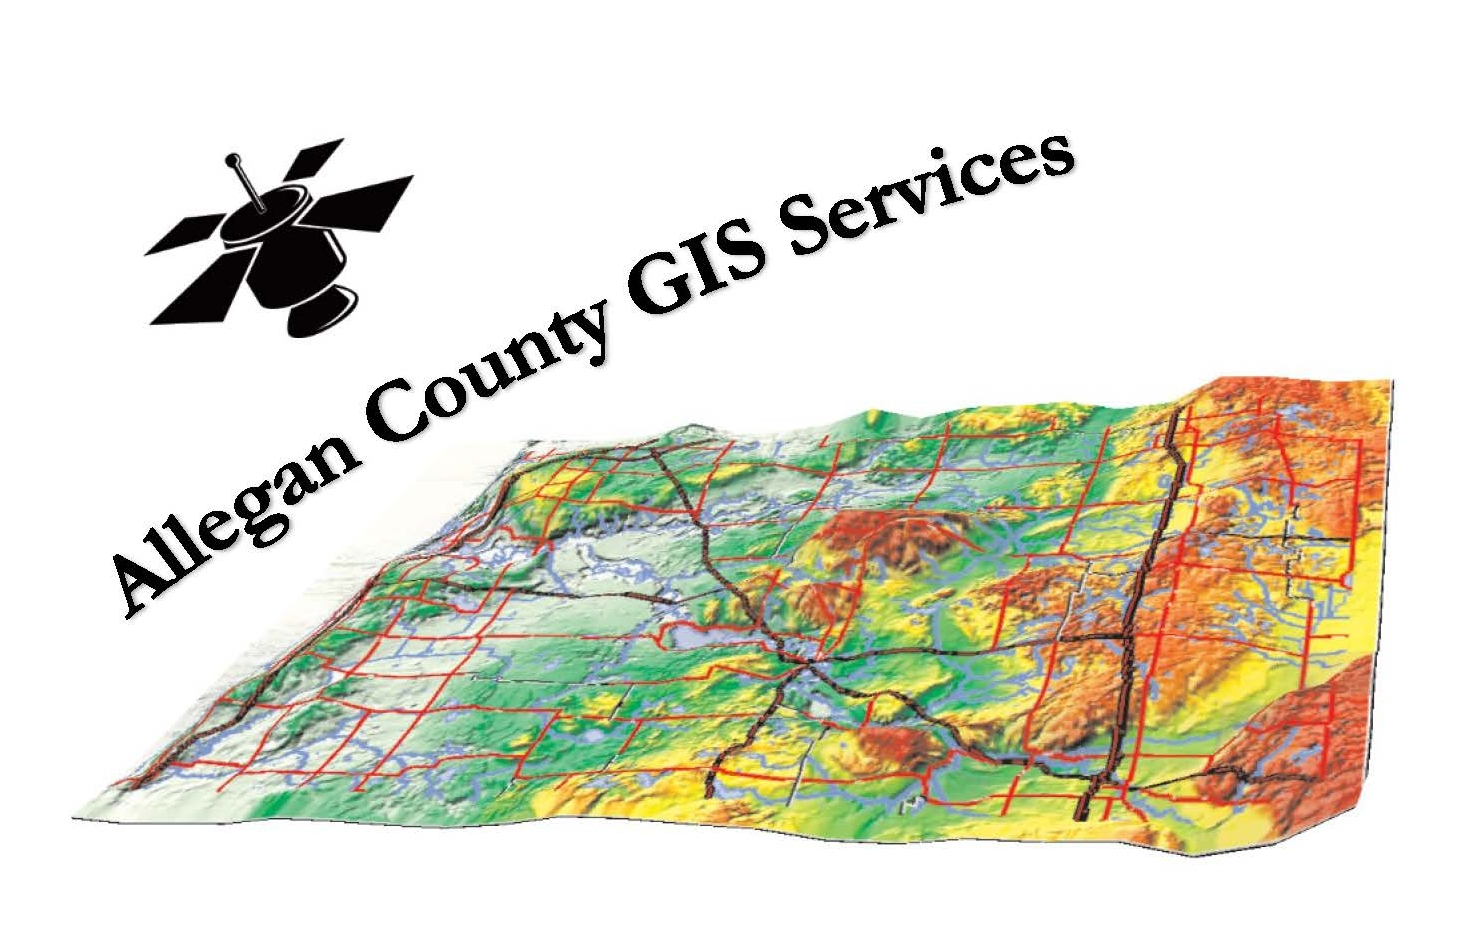
\includegraphics[scale=.45]{GIS_Logo_better.jpg}
\end{center}
\end{figure}
\Huge \bfseries \titlename \\ % Title text
\HRule \\[.4cm] % Horizontal Line added
\author{\Large Allegan County GIS \\\Large www.allegancounty.org/gis} % defines author
}  % inputs common title

\begin{document}% document begins

\ifstandalone
\maketitle % creates title page
\clearpage
\tableofcontents % creates TOC
\clearpage
\fi

\subsection{Forfeiture Data Collection}

\subsubsection{Problem and Analysis}

\paragraph{Background\\}
Treasurer department has an annual responsibility to properly document the tax forfeiture process.  The LIS Department built an application in MS Access and MapInfo that consumed a daily export from BSA and was deployed to the field on a laptop.  A digital camera was used for site photos and later imported into the laptop.

\paragraph{Statement of Problem\\}
Current Tax Forfeiture workflow is built on MapInfo software which has been replaced by ESRI software.  The Forfeiture data collection application must be recreated in the ESRI framework.


\paragraph{Analysis\\}
Tax Forfeiture Application will facilitate:

\begin{itemize} %1

\item Mobile data collection on handheld device via Collector for ArcGIS configured with Allegan County GIS Portal  (\textbf{device app})

\begin{itemize} %2

\item Device app will:

\begin{itemize} %3

\item Synchronize with data in the office (online)
\item Navigate to forfeiture sites (offline)
\item Collect data and photos of forfeiture sites (offline)
\item Synchronize the collected data with data in the office (online)
\end{itemize} %3

\end{itemize} %2

\item Daily form production and printing for each site visited with required data and images.

\end{itemize} %1

\clearpage
\subsubsection{Design}

\paragraph{Forfeiture Data Collection\\}
Three parts of the daily routine:

\begin{enumerate}

\item Pre-processing (in the office):
\begin{itemize}

\item Export current forfeiture list from BSA
\item Update webmap layers with results from BSA export
\item Synchronize from webmap layers to field collection device \textbf{(device app)}
\end{itemize}

\item Field data collection with device app:
\begin{itemize}

\item Support navigation to forfeiture sites
\item Provide a checklist of data points about the site
\item Attach photos to the site
\item Save results for synchronization in post-processing
\end{itemize}

\item Post-processing (in the office)
\begin{itemize}

\item Synchronize data and images collected in device app to webmap layers

\end{itemize}
\end{enumerate}

\paragraph{Backend Data Details\\\\}
%feature class : ForfetureParcels

\begin{minipage}{0.4\textwidth}
\begin{itemize}
\item[\textbf{ForfeitureParcels}]Dat is in 
\end{itemize}
\end{minipage}%
%
\begin{minipage}{0.4\textwidth}
\begin{center}
    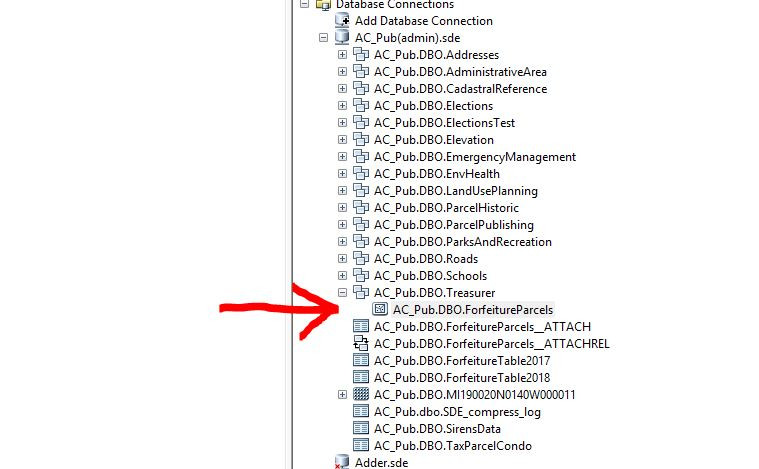
\includegraphics[width=0.6\textwidth]{ForfParcelsCatalog2}
    \captionof{figure}{live data}
    \label{img:g}
\end{center}
\end{minipage}

\subparagraph{ForfeitureParcels Feature Class\\}
Details about the data
\clearpage
\paragraph{Collector Setup Details\\}
Install Collector for ArcGIS from Google Play Store

\clearpage
\subsubsection{Hard Copy Record}
\clearpage
\subsubsection{User Manual}
\clearpage
\subsubsection{Software}
\clearpage
\end{document}